\documentclass[border=0.1cm]{standalone}
\usepackage[utf8]{inputenc}

\usepackage{tikz}
\usepackage{amsfonts}
\usepackage{amsmath,amssymb}
\usepackage{systeme,mathtools}
\usetikzlibrary{positioning,arrows.meta,quotes}
\usetikzlibrary{shapes,snakes}
\usetikzlibrary{bayesnet}
\tikzset{>=latex}

\begin{document}
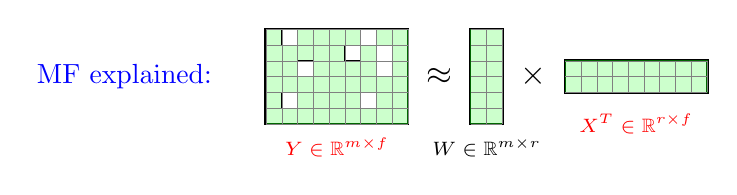
\begin{tikzpicture}
    \draw (-1.8,0.6) node {{\color{blue}MF explained:}};
    \draw [very thick] (0,0) rectangle (3.6/2,2.4/2);
    \filldraw [fill=green!20!white,draw=green!40!black] (0,0) rectangle (3.6/2,2.4/2);
    \filldraw [fill=white] (0.4/2,0.4/2) rectangle (0.8/2,0.8/2);
    \filldraw [fill=white] (2.4/2,0.4/2) rectangle (2.8/2,0.8/2);
    \filldraw [fill=white] (0.8/2,1.2/2) rectangle (1.2/2,1.6/2);
    \filldraw [fill=white] (2.0/2,1.6/2) rectangle (2.4/2,2.0/2);
    \filldraw [fill=white] (0.4/2,2.0/2) rectangle (0.8/2,2.4/2);
    \filldraw [fill=white] (2.4/2,2.0/2) rectangle (2.8/2,2.4/2);
    \filldraw [fill=white] (2.8/2,1.2/2) rectangle (3.2/2,2.0/2);
    \draw [step=0.4/2, very thin, color=gray] (0,0) grid (3.6/2,2.4/2);
    \draw (1.8/2,-0.3) node {{\color{red}\scriptsize{$Y\in\mathbb{R}^{m\times f}$}}};
    \draw (4.4/2,1.2/2) node {{\color{black}\large{$\approx$}}};
    \draw [very thick] (5.2/2,0) rectangle (6.0/2,2.4/2);
    \filldraw [fill=green!20!white,draw=green!40!black] (5.2/2,0) rectangle (6.0/2,2.4/2);
    \draw [step=0.4/2, very thin, color=gray] (5.2/2,0) grid (6.0/2,2.4/2);
    \draw (5.6/2,-0.3) node {{\color{black}\scriptsize{$W\in\mathbb{R}^{m\times r}$}}};
    \draw (6.8/2,1.2/2) node {{\color{black}\large{$\times$}}};
    \draw [very thick] (7.6/2,0.8/2) rectangle (11.2/2,1.6/2);
    \filldraw [fill=green!20!white,draw=green!40!black] (7.6/2,0.8/2) rectangle (11.2/2,1.6/2);
    \draw [step=0.4/2, very thin, color=gray] (7.6/2,0.8/2) grid (11.2/2,1.6/2);
    \draw (9.4/2,0) node {{\color{red}\scriptsize{$X^{T}\in\mathbb{R}^{r\times f}$}}};
\end{tikzpicture}
\end{document}